\documentclass{article}

% if you need to pass options to natbib, use, e.g.:
%     \PassOptionsToPackage{numbers, compress}{natbib}
% before loading neurips_2021

% ready for submission
% \usepackage{neurips_2021}

% to compile a preprint version, e.g., for submission to arXiv, add add the
% [preprint] option:
    \usepackage[preprint]{neurips_2021}

% to compile a camera-ready version, add the [final] option, e.g.:
%     \usepackage[final]{neurips_2021}

% to avoid loading the natbib package, add option nonatbib:
%    \usepackage[nonatbib]{neurips_2021}

\usepackage[utf8]{inputenc} % allow utf-8 input
\usepackage[T1]{fontenc}    % use 8-bit T1 fonts
\usepackage{hyperref}       % hyperlinks
\usepackage{url}            % simple URL typesetting
\usepackage{booktabs}       % professional-quality tables
\usepackage{amsfonts}       % blackboard math symbols
\usepackage{nicefrac}       % compact symbols for 1/2, etc.
\usepackage{microtype}      % microtypography
\usepackage{xcolor}         % colors
\usepackage{graphicx}
\usepackage{float}
\usepackage{hyperref}

\title{CSE 151B Project Final Report}

% The \author macro works with any number of authors. There are two commands
% used to separate the names and addresses of multiple authors: \And and \AND.
%
% Using \And between authors leaves it to LaTeX to determine where to break the
% lines. Using \AND forces a line break at that point. So, if LaTeX puts 3 of 4
% authors names on the first line, and the last on the second line, try using
% \AND instead of \And before the third author name.

\author{%
  Alexander Friend \\
  \texttt{apfriend@ucsd.edu} \\
}

\begin{document}

  \maketitle

  \section{Task Description and Exploratory Analysis}
    \subsection{Problem A [0.5 points]}
        
      \textbf{Describe in your own words what the deep learning task is and
      why it is important. Provide some real-world examples where solving this task can have
      great impact on our daily life and the society.}
    
    \subsection{Problem B [0.5 points]}

      \textbf{Use \href{https://scholar.google.com/}{Google Scholar} or other internet resources to research on
      this task. What type of methods have been examined before? Include some references and
      discuss their ideas in a few sentences. You can use 
      \href{https://www.overleaf.com/learn/latex/Bibliography_management_with_bibtex}{Bibtex} 
      to manage your bibliography.}

    \subsection{Problem C [1 points]}        

      \textbf{Define the input and output in mathematical language and formu-
      late your prediction task. From the abstraction, do you think your model can potentially
      solve other tasks beyond this project? If so, list some examples and explain your rationale.}
              
  \section{Exploratory Data Analysis}

  \section{Deep Learning Model}
  \label{gen_inst}
    \subsection{Problem A [1 Points]}
      Thus far my best performing model is a PyTorch linear neural net running in an Anaconda environment.
      The platform I am currently working in is my local machine running Ubuntu 20.04 with a 4-core 4-thread Intel i7-7600k CPU 
      running at 4.2 GHz, a GTX 1070 GPU with a max clock speed of 1721 MHz and 8 GB of GDDR5 memory, and 16 GB of 3000 MHz DDR4 memory.
      
      For my initial baseline model I made a simple single layer linear neural network, using Adam as an optimizer And
      and mean square error as my loss function. I used a learning rate of 0.001, and  trained my best model for
      10 epochs. Each epoch took approximately 3 minutes to train.
      
      I chose mean square error as it increases the penalty for worse predictions, compared to a optimizer like
      mean absolute error, which penalizes with a linear rate. 
      
      In order to get the correct outputs from my trained model, I sliced the output prediction tensors so as to only
      keep the first inner 2 elements of each tensor (the predicted x and y coordinates), and then selected the correct car based on
      each inputs  {\fontfamily{qcr}\selectfont agent\_id}.

    \subsection{Problem B [1 Points]}        
      I experimented with multilayer linear models and an LSTM model as well, however these actually performed worse on 
      the validation set once I uploaded them to Kaggle. Thus far, the best performing model is a linear one, which
      takes in the assumption that cars will be moving at about the same rate over the 5 seconds period of training and prediction.
      
  \section{Experiment Results and Future Work}
  \label{headings}
    \subsection{Problem A [1 points]}
          
      \begin{figure}[H]
          \centering
          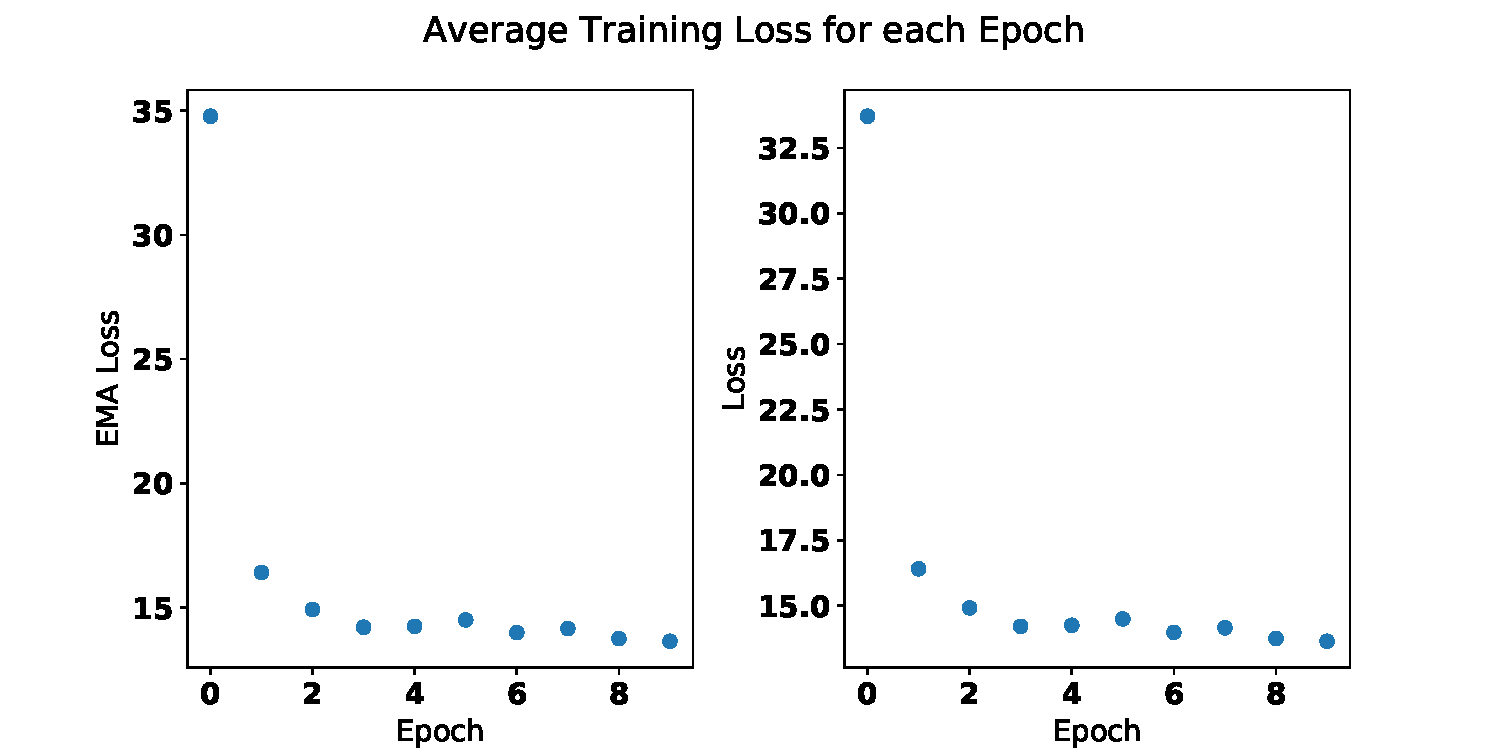
\includegraphics[height=6cm]{figures/train-loss/2021.05.24-multi-linear-ema075-epoch10-batchsz128-epoch-avg.pdf}%
          \caption{Plot of the average training mean square error for my best perfoming single layer model}%
          \label{fig:5}
      \end{figure}
      
      This model however achieved a significantly lower loss on the training set compared to the final validation set on Kaggle,
      suggesting that my model has overfit the training data. This means that a more complex model with more variance will need to be implemented.
      
      Based on my lack of success with an LSTM approach, I will continue to work on more complex linear models, as well as trying other architetures
      such as a RNN model, which may achieve a better result as it can take into account previous training examples.
      
      My current rank on the Kaggle leaderboard is 40 out of 57.

  \appendix

  \section{Appendix}

  \url{https://github.com/apfriend/cse151b-kaggle.git}

        
\end{document}